The objective of this section is to establish the quantitative relationship between different neural network hyperparameters; namely: the number of nodes ($n_{nodes}$), the number of neurons ($n_{neurons}$), the number of experiments ($n_{experiments}$) and the number of layers ($n_{layers}$), and how the affect the neural network predictive performance. 

In order to study how these hyperparameters impact the performance of the machine learning model, we have decided to establish two finite element models that will act as ground-truth to compare against. First, a simple dielectric elastomer with 4 electrodes is analysed, followed by a complex 20 electrode FE model. 

To measure the accuracy of the prediction made by the neural network, the R2 metric is used. 

\begin{equation}
  \mbox{R2} = 1 - \dfrac{\sum ( y - y')^2}{\sum (y - \hat{y})^2}
  \label{eq:R2_measurement}
\end{equation}

\subsection{First test case: 4-electrode dielectric elastomer}


The first ground-truth finite element example is a dielectric elastomer with 4 electrodes embedded: 2 electrodes at the top and 2 electrodes at the middle layer:

\begin{figure}[!ht]
\centering
\resizebox{0.6\textwidth}{!}{%
\begin{circuitikz}
\tikzstyle{every node}=[font=\normalsize]
\draw  (6.25,13.75) rectangle (6.25,13.75);
\draw [ color={rgb,255:red,28; green,113; blue,216} , fill={rgb,255:red,255; green,190; blue,111}] (9.75,15.75) -- (7,15.75) -- (5,13.75) -- (7.75,13.75) -- cycle;
\draw [ color={rgb,255:red,28; green,113; blue,216} , fill={rgb,255:red,255; green,120; blue,0}] (3.5,11.75) -- (5.75,11.75) -- (7.75,13.75) -- (5.5,13.75) -- cycle;
\draw (3.5,12.25) to[short] (7.5,16.25);
\draw (3.5,12.25) to[short] (5.75,12.25);
\draw (5.75,12.25) to[short] (9.75,16.25);
\draw (7.5,16.25) to[short] (9.75,16.25);
\draw  (6.25,13.25) rectangle (6.25,13.25);
\draw (3.5,11.75) to[short] (5.75,11.75);
\draw (5.75,11.75) to[short] (9.75,15.75);
\draw (9.25,15.75) to[short] (9.75,15.75);
\draw  (6.25,12.75) rectangle (6.25,12.75);
\draw (3.5,11.25) to[short] (5.75,11.25);
\draw (5.75,11.25) to[short] (9.75,15.25);
\draw (3.5,12.25) to[short] (3.5,11.25);
\draw (5.75,12.25) to[short] (5.75,11.25);
\draw (9.75,16.25) to[short] (9.75,15.25);
\draw (5.5,14.25) to[short] (7.75,14.25);
\draw [dashed] (9.25,15.75) -- (7.5,15.75);
\draw [dashed] (3.5,11.75) -- (7.5,15.75);
\draw [dashed] (5.5,13.75) -- (7.25,13.75);
\draw [short] (7.25,13.75) -- (7.75,13.75);
\node [font=\normalsize, color={rgb,255:red,28; green,113; blue,216}] at (3.5,13.75) {Electrode 1};
\node [font=\normalsize, color={rgb,255:red,98; green,160; blue,234}] at (5.5,16) {Electrode 2};
\node [font=\normalsize, color={rgb,255:red,255; green,163; blue,72}] at (10.25,14) {Electrode 4};
\node [font=\normalsize, color={rgb,255:red,255; green,120; blue,0}] at (7.75,11.75) {Electrode 3};
\draw [ color={rgb,255:red,28; green,113; blue,216} , fill={rgb,255:red,53; green,132; blue,228}] (3.5,12.25) -- (5.75,12.25) -- (7.75,14.25) -- (5.5,14.25) -- cycle;
\draw  (9,13.75) rectangle (9,13.75);
\draw [ color={rgb,255:red,28; green,113; blue,216} , fill={rgb,255:red,153; green,193; blue,241}] (5.5,14.25) -- (7.75,14.25) -- (9.75,16.25) -- (7.5,16.25) -- cycle;
\draw (9.75,16.25) to[short] (10.25,16.75);
\draw (9.75,16.25) to[short] (10.25,16.5);
\draw (9.75,16.25) to[short] (10,16.75);
\draw (10,16.75) to[short] (10.25,16.75);
\draw (10.25,16.75) to[short] (10.25,16.5);
\draw (9.75,15.25) to[short] (10.25,15.75);
\draw (9.75,15.25) to[short] (10.25,15.5);
\draw (9.75,15.25) to[short] (10,15.75);
\draw (10,15.75) to[short] (10.25,15.75);
\draw (10.25,15.75) to[short] (10.25,15.5);
\draw [ fill={rgb,255:red,94; green,92; blue,100} ] (10,15.75) rectangle (10.25,15.5);
\draw (9.75,15.75) to[short] (10.25,16.25);
\draw (9.75,15.75) to[short] (10.25,16);
\draw (9.75,15.75) to[short] (10,16.25);
\draw (10,16.25) to[short] (10.25,16.25);
\draw (10.25,16.25) to[short] (10.25,16);
\draw [ fill={rgb,255:red,94; green,92; blue,100} ] (10,16.25) rectangle (10.25,16);
\draw (7.5,16.25) to[short] (8,16.75);
\draw (7.5,16.25) to[short] (8,16.5);
\draw (7.5,16.25) to[short] (7.75,16.75);
\draw (7.75,16.75) to[short] (8,16.75);
\draw (8,16.75) to[short] (8,16.5);
\draw [ fill={rgb,255:red,94; green,92; blue,100} ] (7.75,16.75) rectangle (8,16.5);
\draw (8.5,16.25) to[short] (9,16.75);
\draw (8.5,16.25) to[short] (9,16.5);
\draw (8.5,16.25) to[short] (8.75,16.75);
\draw (8.75,16.75) to[short] (9,16.75);
\draw (9,16.75) to[short] (9,16.5);
\draw [ fill={rgb,255:red,119; green,118; blue,123} ] (8.75,16.75) rectangle (9,16.5);
\draw [ fill={rgb,255:red,94; green,92; blue,100} ] (10,16.75) rectangle (10.25,16.5);
\node [font=\normalsize] at (9,17.25) {Fixed face};
\end{circuitikz}
}%

\label{fig:my_label}
\end{figure}

Different combinations of potential in each electrode will cause an unique deformation shape. For example, when the potential in electrode 1 and 2 are equal and the potential in electrode 3 and 4 are 0, a bending will be induced in the dielectric. More exotic combinations of potentials will induce a combination of bending and torsion, which can cause severe displacements, depending on the overall thickness of the dielectric and magnitude of the potentials. 

To study these types of varying deformations, a Design of Experiments (DoE) will be employed using a Latin Hypercube Sampling algorithm. The main idea behind this is that each of the electrodes can have a varying potential between 0 and 0.3 V. With a fixed potential in each of the electrodes, $n$ number of sampling points will be created by varying the potential in the rest of the electrodes. A finite number of combinations ($n\times n_{variables}\times 2$) will be created, so that no electrode has the same potential using the Latin Hypercube algorithm. This effect can be visualized using 2 variables in a 3D cube:





\tikzset{every picture/.style={line width=0.75pt}} %set default line width to 0.75pt        

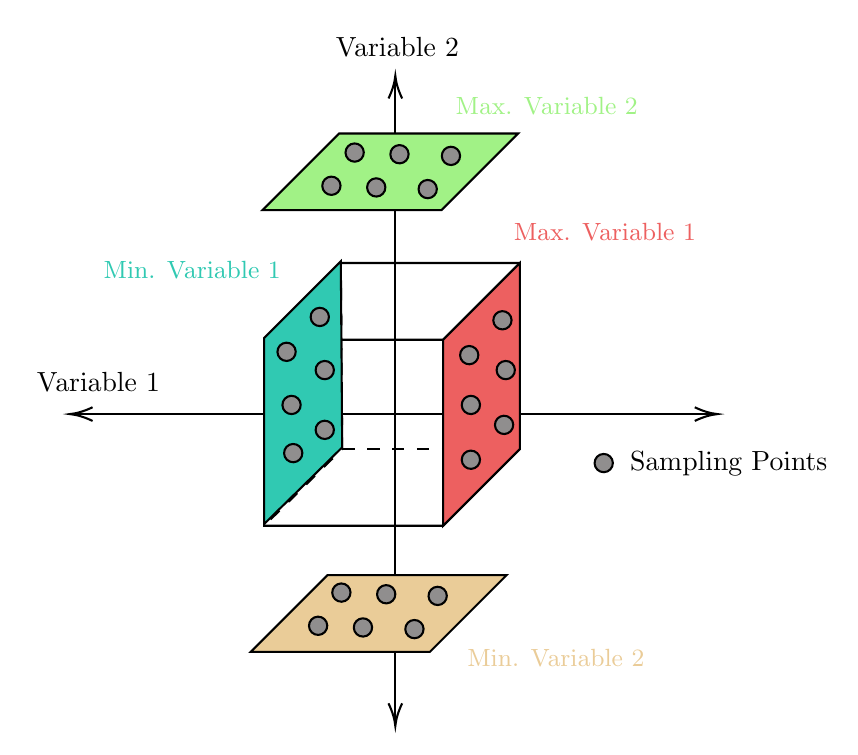
\begin{tikzpicture}[x=0.75pt,y=0.75pt,yscale=-1,xscale=1]
%uncomment if require: \path (0,426); %set diagram left start at 0, and has height of 426

%Shape: Cube [id:dp41916472639407576] 
\draw   (188.8,213.17) -- (225.77,176.2) -- (312.03,176.2) -- (312.03,265.83) -- (275.06,302.8) -- (188.8,302.8) -- cycle ; \draw   (312.03,176.2) -- (275.06,213.17) -- (188.8,213.17) ; \draw   (275.06,213.17) -- (275.06,302.8) ;
%Straight Lines [id:da1100678834838219] 
\draw    (254.4,249) -- (405.23,249) ;
\draw [shift={(407.23,249)}, rotate = 180] [color={rgb, 255:red, 0; green, 0; blue, 0 }  ][line width=0.75]    (10.93,-3.29) .. controls (6.95,-1.4) and (3.31,-0.3) .. (0,0) .. controls (3.31,0.3) and (6.95,1.4) .. (10.93,3.29)   ;
%Straight Lines [id:da8209310669516441] 
\draw    (254.4,249) -- (97.23,249) ;
\draw [shift={(95.23,249)}, rotate = 360] [color={rgb, 255:red, 0; green, 0; blue, 0 }  ][line width=0.75]    (10.93,-3.29) .. controls (6.95,-1.4) and (3.31,-0.3) .. (0,0) .. controls (3.31,0.3) and (6.95,1.4) .. (10.93,3.29)   ;
%Shape: Polygon [id:ds315102272045769] 
\draw  [dash pattern={on 4.5pt off 4.5pt}] (225.77,176.2) -- (226.43,265.83) -- (188.8,302.8) -- (188.8,213.17) -- cycle ;
%Straight Lines [id:da6924249131024756] 
\draw  [dash pattern={on 4.5pt off 4.5pt}]  (226.43,265.83) -- (312.03,265.83) ;
%Shape: Polygon [id:ds26648827466781355] 
\draw  [fill={rgb, 255:red, 237; green, 96; blue, 96 }  ,fill opacity=1 ] (312.03,176.2) -- (312.03,265.83) -- (275.06,302.8) -- (275.06,213.17) -- cycle ;
%Shape: Polygon [id:ds5376783951801227] 
\draw  [fill={rgb, 255:red, 48; green, 201; blue, 178 }  ,fill opacity=1 ] (225.77,175.4) -- (226.43,265.03) -- (188.8,302) -- (188.8,212.37) -- cycle ;
%Shape: Circle [id:dp6613928021845482] 
\draw  [fill={rgb, 255:red, 144; green, 142; blue, 142 }  ,fill opacity=1 ] (211.23,202.31) .. controls (211.16,199.88) and (213.08,197.85) .. (215.51,197.79) .. controls (217.95,197.72) and (219.97,199.64) .. (220.04,202.07) .. controls (220.1,204.51) and (218.19,206.53) .. (215.75,206.6) .. controls (213.32,206.66) and (211.29,204.75) .. (211.23,202.31) -- cycle ;
%Shape: Circle [id:dp10792302470599302] 
\draw  [fill={rgb, 255:red, 144; green, 142; blue, 142 }  ,fill opacity=1 ] (195.23,219.11) .. controls (195.16,216.68) and (197.08,214.65) .. (199.51,214.59) .. controls (201.95,214.52) and (203.97,216.44) .. (204.04,218.87) .. controls (204.1,221.31) and (202.19,223.33) .. (199.75,223.4) .. controls (197.32,223.46) and (195.29,221.55) .. (195.23,219.11) -- cycle ;
%Shape: Circle [id:dp764393572474829] 
\draw  [fill={rgb, 255:red, 144; green, 142; blue, 142 }  ,fill opacity=1 ] (213.63,227.91) .. controls (213.56,225.48) and (215.48,223.45) .. (217.91,223.39) .. controls (220.35,223.32) and (222.37,225.24) .. (222.44,227.67) .. controls (222.5,230.11) and (220.59,232.13) .. (218.15,232.2) .. controls (215.72,232.26) and (213.69,230.35) .. (213.63,227.91) -- cycle ;
%Shape: Circle [id:dp2635654509882438] 
\draw  [fill={rgb, 255:red, 144; green, 142; blue, 142 }  ,fill opacity=1 ] (197.63,244.71) .. controls (197.56,242.28) and (199.48,240.25) .. (201.91,240.19) .. controls (204.35,240.12) and (206.37,242.04) .. (206.44,244.47) .. controls (206.5,246.91) and (204.59,248.93) .. (202.15,249) .. controls (199.72,249.06) and (197.69,247.15) .. (197.63,244.71) -- cycle ;
%Shape: Circle [id:dp720401298117804] 
\draw  [fill={rgb, 255:red, 144; green, 142; blue, 142 }  ,fill opacity=1 ] (213.63,256.71) .. controls (213.56,254.28) and (215.48,252.25) .. (217.91,252.19) .. controls (220.35,252.12) and (222.37,254.04) .. (222.44,256.47) .. controls (222.5,258.91) and (220.59,260.93) .. (218.15,261) .. controls (215.72,261.06) and (213.69,259.15) .. (213.63,256.71) -- cycle ;
%Shape: Circle [id:dp3334941876745968] 
\draw  [fill={rgb, 255:red, 144; green, 142; blue, 142 }  ,fill opacity=1 ] (198.43,267.91) .. controls (198.36,265.48) and (200.28,263.45) .. (202.71,263.39) .. controls (205.15,263.32) and (207.17,265.24) .. (207.24,267.67) .. controls (207.3,270.11) and (205.39,272.13) .. (202.95,272.2) .. controls (200.52,272.26) and (198.49,270.35) .. (198.43,267.91) -- cycle ;
%Shape: Circle [id:dp9121056350905267] 
\draw  [fill={rgb, 255:red, 144; green, 142; blue, 142 }  ,fill opacity=1 ] (299.23,203.91) .. controls (299.16,201.48) and (301.08,199.45) .. (303.51,199.39) .. controls (305.95,199.32) and (307.97,201.24) .. (308.04,203.67) .. controls (308.1,206.11) and (306.19,208.13) .. (303.75,208.2) .. controls (301.32,208.26) and (299.29,206.35) .. (299.23,203.91) -- cycle ;
%Shape: Circle [id:dp461002915724564] 
\draw  [fill={rgb, 255:red, 144; green, 142; blue, 142 }  ,fill opacity=1 ] (283.23,220.71) .. controls (283.16,218.28) and (285.08,216.25) .. (287.51,216.19) .. controls (289.95,216.12) and (291.97,218.04) .. (292.04,220.47) .. controls (292.1,222.91) and (290.19,224.93) .. (287.75,225) .. controls (285.32,225.06) and (283.29,223.15) .. (283.23,220.71) -- cycle ;
%Shape: Circle [id:dp715936866594871] 
\draw  [fill={rgb, 255:red, 144; green, 142; blue, 142 }  ,fill opacity=1 ] (300.83,227.91) .. controls (300.76,225.48) and (302.68,223.45) .. (305.11,223.39) .. controls (307.55,223.32) and (309.57,225.24) .. (309.64,227.67) .. controls (309.7,230.11) and (307.79,232.13) .. (305.35,232.2) .. controls (302.92,232.26) and (300.89,230.35) .. (300.83,227.91) -- cycle ;
%Shape: Circle [id:dp5335650842060755] 
\draw  [fill={rgb, 255:red, 144; green, 142; blue, 142 }  ,fill opacity=1 ] (284.03,244.71) .. controls (283.96,242.28) and (285.88,240.25) .. (288.31,240.19) .. controls (290.75,240.12) and (292.77,242.04) .. (292.84,244.47) .. controls (292.9,246.91) and (290.99,248.93) .. (288.55,249) .. controls (286.12,249.06) and (284.09,247.15) .. (284.03,244.71) -- cycle ;
%Shape: Circle [id:dp6761023350021587] 
\draw  [fill={rgb, 255:red, 144; green, 142; blue, 142 }  ,fill opacity=1 ] (300.03,254.31) .. controls (299.96,251.88) and (301.88,249.85) .. (304.31,249.79) .. controls (306.75,249.72) and (308.77,251.64) .. (308.84,254.07) .. controls (308.9,256.51) and (306.99,258.53) .. (304.55,258.6) .. controls (302.12,258.66) and (300.09,256.75) .. (300.03,254.31) -- cycle ;
%Shape: Circle [id:dp7779527390505632] 
\draw  [fill={rgb, 255:red, 144; green, 142; blue, 142 }  ,fill opacity=1 ] (284.03,271.11) .. controls (283.96,268.68) and (285.88,266.65) .. (288.31,266.59) .. controls (290.75,266.52) and (292.77,268.44) .. (292.84,270.87) .. controls (292.9,273.31) and (290.99,275.33) .. (288.55,275.4) .. controls (286.12,275.46) and (284.09,273.55) .. (284.03,271.11) -- cycle ;
%Shape: Circle [id:dp39193327346815965] 
\draw  [fill={rgb, 255:red, 144; green, 142; blue, 142 }  ,fill opacity=1 ] (348.03,272.71) .. controls (347.96,270.28) and (349.88,268.25) .. (352.31,268.19) .. controls (354.75,268.12) and (356.77,270.04) .. (356.84,272.47) .. controls (356.9,274.91) and (354.99,276.93) .. (352.55,277) .. controls (350.12,277.06) and (348.09,275.15) .. (348.03,272.71) -- cycle ;
%Straight Lines [id:da4370737882051544] 
\draw    (252.03,397.29) -- (252.03,88) ;
\draw [shift={(252.03,86)}, rotate = 90] [color={rgb, 255:red, 0; green, 0; blue, 0 }  ][line width=0.75]    (10.93,-3.29) .. controls (6.95,-1.4) and (3.31,-0.3) .. (0,0) .. controls (3.31,0.3) and (6.95,1.4) .. (10.93,3.29)   ;
\draw [shift={(252.03,399.29)}, rotate = 270] [color={rgb, 255:red, 0; green, 0; blue, 0 }  ][line width=0.75]    (10.93,-3.29) .. controls (6.95,-1.4) and (3.31,-0.3) .. (0,0) .. controls (3.31,0.3) and (6.95,1.4) .. (10.93,3.29)   ;
%Shape: Polygon [id:ds027192625551482386] 
\draw  [fill={rgb, 255:red, 161; green, 242; blue, 134 }  ,fill opacity=1 ] (311.23,113.8) -- (274.26,150.77) -- (188,150.77) -- (224.97,113.8) -- cycle ;
%Shape: Polygon [id:ds7003641159858384] 
\draw  [fill={rgb, 255:red, 234; green, 204; blue, 152 }  ,fill opacity=1 ] (305.63,326.6) -- (268.66,363.57) -- (182.4,363.57) -- (219.37,326.6) -- cycle ;
%Shape: Circle [id:dp7862884715493691] 
\draw  [fill={rgb, 255:red, 144; green, 142; blue, 142 }  ,fill opacity=1 ] (228.03,123.11) .. controls (227.96,120.68) and (229.88,118.65) .. (232.31,118.59) .. controls (234.75,118.52) and (236.77,120.44) .. (236.84,122.87) .. controls (236.9,125.31) and (234.99,127.33) .. (232.55,127.4) .. controls (230.12,127.46) and (228.09,125.55) .. (228.03,123.11) -- cycle ;
%Shape: Circle [id:dp9269233874737624] 
\draw  [fill={rgb, 255:red, 144; green, 142; blue, 142 }  ,fill opacity=1 ] (216.83,139.11) .. controls (216.76,136.68) and (218.68,134.65) .. (221.11,134.59) .. controls (223.55,134.52) and (225.57,136.44) .. (225.64,138.87) .. controls (225.7,141.31) and (223.79,143.33) .. (221.35,143.4) .. controls (218.92,143.46) and (216.89,141.55) .. (216.83,139.11) -- cycle ;
%Shape: Circle [id:dp9900121536496537] 
\draw  [fill={rgb, 255:red, 144; green, 142; blue, 142 }  ,fill opacity=1 ] (249.63,123.91) .. controls (249.56,121.48) and (251.48,119.45) .. (253.91,119.39) .. controls (256.35,119.32) and (258.37,121.24) .. (258.44,123.67) .. controls (258.5,126.11) and (256.59,128.13) .. (254.15,128.2) .. controls (251.72,128.26) and (249.69,126.35) .. (249.63,123.91) -- cycle ;
%Shape: Circle [id:dp0010559062693412669] 
\draw  [fill={rgb, 255:red, 144; green, 142; blue, 142 }  ,fill opacity=1 ] (238.43,139.91) .. controls (238.36,137.48) and (240.28,135.45) .. (242.71,135.39) .. controls (245.15,135.32) and (247.17,137.24) .. (247.24,139.67) .. controls (247.3,142.11) and (245.39,144.13) .. (242.95,144.2) .. controls (240.52,144.26) and (238.49,142.35) .. (238.43,139.91) -- cycle ;
%Shape: Circle [id:dp9729939432021396] 
\draw  [fill={rgb, 255:red, 144; green, 142; blue, 142 }  ,fill opacity=1 ] (274.43,124.71) .. controls (274.36,122.28) and (276.28,120.25) .. (278.71,120.19) .. controls (281.15,120.12) and (283.17,122.04) .. (283.24,124.47) .. controls (283.3,126.91) and (281.39,128.93) .. (278.95,129) .. controls (276.52,129.06) and (274.49,127.15) .. (274.43,124.71) -- cycle ;
%Shape: Circle [id:dp5583563494601032] 
\draw  [fill={rgb, 255:red, 144; green, 142; blue, 142 }  ,fill opacity=1 ] (263.23,140.71) .. controls (263.16,138.28) and (265.08,136.25) .. (267.51,136.19) .. controls (269.95,136.12) and (271.97,138.04) .. (272.04,140.47) .. controls (272.1,142.91) and (270.19,144.93) .. (267.75,145) .. controls (265.32,145.06) and (263.29,143.15) .. (263.23,140.71) -- cycle ;
%Shape: Circle [id:dp2803403187081903] 
\draw  [fill={rgb, 255:red, 144; green, 142; blue, 142 }  ,fill opacity=1 ] (221.63,335.11) .. controls (221.56,332.68) and (223.48,330.65) .. (225.91,330.59) .. controls (228.35,330.52) and (230.37,332.44) .. (230.44,334.87) .. controls (230.5,337.31) and (228.59,339.33) .. (226.15,339.4) .. controls (223.72,339.46) and (221.69,337.55) .. (221.63,335.11) -- cycle ;
%Shape: Circle [id:dp08580816994108764] 
\draw  [fill={rgb, 255:red, 144; green, 142; blue, 142 }  ,fill opacity=1 ] (210.43,351.11) .. controls (210.36,348.68) and (212.28,346.65) .. (214.71,346.59) .. controls (217.15,346.52) and (219.17,348.44) .. (219.24,350.87) .. controls (219.3,353.31) and (217.39,355.33) .. (214.95,355.4) .. controls (212.52,355.46) and (210.49,353.55) .. (210.43,351.11) -- cycle ;
%Shape: Circle [id:dp8920356550311489] 
\draw  [fill={rgb, 255:red, 144; green, 142; blue, 142 }  ,fill opacity=1 ] (243.23,335.91) .. controls (243.16,333.48) and (245.08,331.45) .. (247.51,331.39) .. controls (249.95,331.32) and (251.97,333.24) .. (252.04,335.67) .. controls (252.1,338.11) and (250.19,340.13) .. (247.75,340.2) .. controls (245.32,340.26) and (243.29,338.35) .. (243.23,335.91) -- cycle ;
%Shape: Circle [id:dp9149486091931166] 
\draw  [fill={rgb, 255:red, 144; green, 142; blue, 142 }  ,fill opacity=1 ] (232.03,351.91) .. controls (231.96,349.48) and (233.88,347.45) .. (236.31,347.39) .. controls (238.75,347.32) and (240.77,349.24) .. (240.84,351.67) .. controls (240.9,354.11) and (238.99,356.13) .. (236.55,356.2) .. controls (234.12,356.26) and (232.09,354.35) .. (232.03,351.91) -- cycle ;
%Shape: Circle [id:dp453151861693878] 
\draw  [fill={rgb, 255:red, 144; green, 142; blue, 142 }  ,fill opacity=1 ] (268.03,336.71) .. controls (267.96,334.28) and (269.88,332.25) .. (272.31,332.19) .. controls (274.75,332.12) and (276.77,334.04) .. (276.84,336.47) .. controls (276.9,338.91) and (274.99,340.93) .. (272.55,341) .. controls (270.12,341.06) and (268.09,339.15) .. (268.03,336.71) -- cycle ;
%Shape: Circle [id:dp2654623156037197] 
\draw  [fill={rgb, 255:red, 144; green, 142; blue, 142 }  ,fill opacity=1 ] (256.83,352.71) .. controls (256.76,350.28) and (258.68,348.25) .. (261.11,348.19) .. controls (263.55,348.12) and (265.57,350.04) .. (265.64,352.47) .. controls (265.7,354.91) and (263.79,356.93) .. (261.35,357) .. controls (258.92,357.06) and (256.89,355.15) .. (256.83,352.71) -- cycle ;

% Text Node
\draw (108.99,233.5) node   [align=left] {Variable 1};
% Text Node
\draw (279.6,94.6) node [anchor=north west][inner sep=0.75pt]  [font=\small,color={rgb, 255:red, 161; green, 242; blue, 134 }  ,opacity=1 ] [align=left] {Max. Variable 2};
% Text Node
\draw (307.6,155.4) node [anchor=north west][inner sep=0.75pt]  [font=\small,color={rgb, 255:red, 237; green, 96; blue, 96 }  ,opacity=1 ] [align=left] {Max. Variable 1};
% Text Node
\draw (363.6,265.4) node [anchor=north west][inner sep=0.75pt]   [align=left] {Sampling Points};
% Text Node
\draw (252.99,71.9) node   [align=left] {Variable 2};
% Text Node
\draw (110,173.8) node [anchor=north west][inner sep=0.75pt]  [font=\small,color={rgb, 255:red, 48; green, 201; blue, 178 }  ,opacity=1 ] [align=left] {Min. Variable 1};
% Text Node
\draw (285.2,361) node [anchor=north west][inner sep=0.75pt]  [font=\small,color={rgb, 255:red, 234; green, 204; blue, 152 }  ,opacity=1 ] [align=left] {Min. Variable 2};


\end{tikzpicture}




By using $n$ number of design variables, this concept expands to an $n$-dimensional hypercube. This allows us to explore a broader design space, making sure that every point data is meaningful, as it represents a unique combination of potentials. In this paper, we utilized 25 sampling points, ie: there are 25 data points in each of the faces of the cube, creating $4\times 25 \times 2=200$ different combinations of potentials.



% I will take 4 combinations of n_nodes and n_experiments



% n_nodes = 10
% n_experiments=4000
% iter = 5000

%n_nodes = 10 
% n_experiments=2000
% iter = 5000


%n_nodes = 30 
% n_experiments=4000
% iter = 5000

%n_nodes = 30 
% n_experiments=2000
% iter = 5000

% Please add the following required packages to your document preamble:
% \usepackage{multirow}
% Please add the following required packages to your document preamble:
% \usepackage{multirow}
\begin{table}[!hb]

\begin{minipage}{.49\textwidth}

\begin{tabular}{lllllllcc|ccc}
\multicolumn{9}{c|}{\multirow{2}{*}{\begin{tabular}[c]{@{}c@{}}$n_{nodes}=10$\\ $n_{experiments}=4000$\end{tabular}}} & \multicolumn{3}{c}{$n_{neurons}$} \\
\multicolumn{9}{c|}{}                                                                                                 & 10        & 20        & 40        \\ \hline
        &         &         &         &         &         &         & \multirow{4}{*}{\rotatebox{90}{$n_{layers}$}}        & 2        &  0.964        &  0.951        &  0.966        \\
        &         &         &         &         &         &         &                                      & 3        &  0.973        &  0.999       &  0.999        \\
        &         &         &         &         &         &         &                                      & 4        &  0.998        &  0.996        &  0.998        \\
        &         &         &         &         &         &         &                                      & 6        &  0.990       & 0.998       &  0.999      
\end{tabular}



\end{minipage}

\begin{minipage}{.49\textwidth}
\begin{tabular}{lllllllcc|ccc}
\multicolumn{9}{c|}{\multirow{2}{*}{\begin{tabular}[c]{@{}c@{}}$n_{nodes}=10$\\ $n_{experiments}=2000$\end{tabular}}} & \multicolumn{3}{c}{$n_{neurons}$} \\
\multicolumn{9}{c|}{}                                                                                                 & 10        & 20        & 40        \\ \hline
        &         &         &         &         &         &         & \multirow{4}{*}{\rotatebox{90}{$n_{layers}$}}        & 2        &  0.946        & 0.956         &  0.960        \\
        &         &         &         &         &         &         &                                      & 3        &  0.996        &  0.999        &  0.997        \\
        &         &         &         &         &         &         &                                      & 4        &  0.995        & 0.999         & 0.998         \\
        &         &         &         &         &         &         &                                      & 6        & 0.994         & 0.998         &  0.998       
\end{tabular}
\end{minipage}

\begin{minipage}{.49\textwidth}
\begin{tabular}{lllllllcc|ccc}
\multicolumn{9}{c|}{\multirow{2}{*}{\begin{tabular}[c]{@{}c@{}}$n_{nodes}=30$\\ $n_{experiments}=4000$\end{tabular}}} & \multicolumn{3}{c}{$n_{neurons}$} \\
\multicolumn{9}{c|}{}                                                                                                 & 10        & 20        & 40        \\ \hline
        &         &         &         &         &         &         & \multirow{4}{*}{\rotatebox{90}{$n_{layers}$}}        & 2        & 0.932         &   0.950       &  0.964        \\
        &         &         &         &         &         &         &                                      & 3        &  0.990        & 0.994         &  0.997        \\
        &         &         &         &         &         &         &                                      & 4        &  0.992        &  0.997        &  0.999        \\
        &         &         &         &         &         &         &                                      & 6        &  0.991        &  0.996       &        0.998 
\end{tabular}
\end{minipage}

\begin{minipage}{.49\textwidth}
\begin{tabular}{lllllllcc|ccc}
\multicolumn{9}{c|}{\multirow{2}{*}{\begin{tabular}[c]{@{}c@{}}$n_{nodes}=30$\\ $n_{experiments}=2000$\end{tabular}}} & \multicolumn{3}{c}{$n_{neurons}$} \\
\multicolumn{9}{c|}{}                                                                                                 & 10        & 20        & 40        \\ \hline
        &         &         &         &         &         &         & \multirow{4}{*}{\rotatebox{90}{$n_{layers}$}}        & 2        & 0.953         &  0.944        &  0.979        \\
        &         &         &         &         &         &         &                                      & 3        &  0.987        &  0.994        &  0.996        \\
        &         &         &         &         &         &         &                                      & 4        &  0.993        &  0.997        & 0.997         \\
        &         &         &         &         &         &         &                                      & 6        & 0.989         &  0.995        &  0.998       
\end{tabular}
\end{minipage}


\end{table}


The best configuration is a combination of 4 layers, 20 neurons, 2000 experiments, 10 nodes and 5000 iterations with an R2 on the test cases of 0.9994

Here is the output of the displacements predicted by the Neural Network compared against the FE outputs:

\begin{figure}
  \centering
  \subfloat[Displacement in the first axis of the coordenate system]{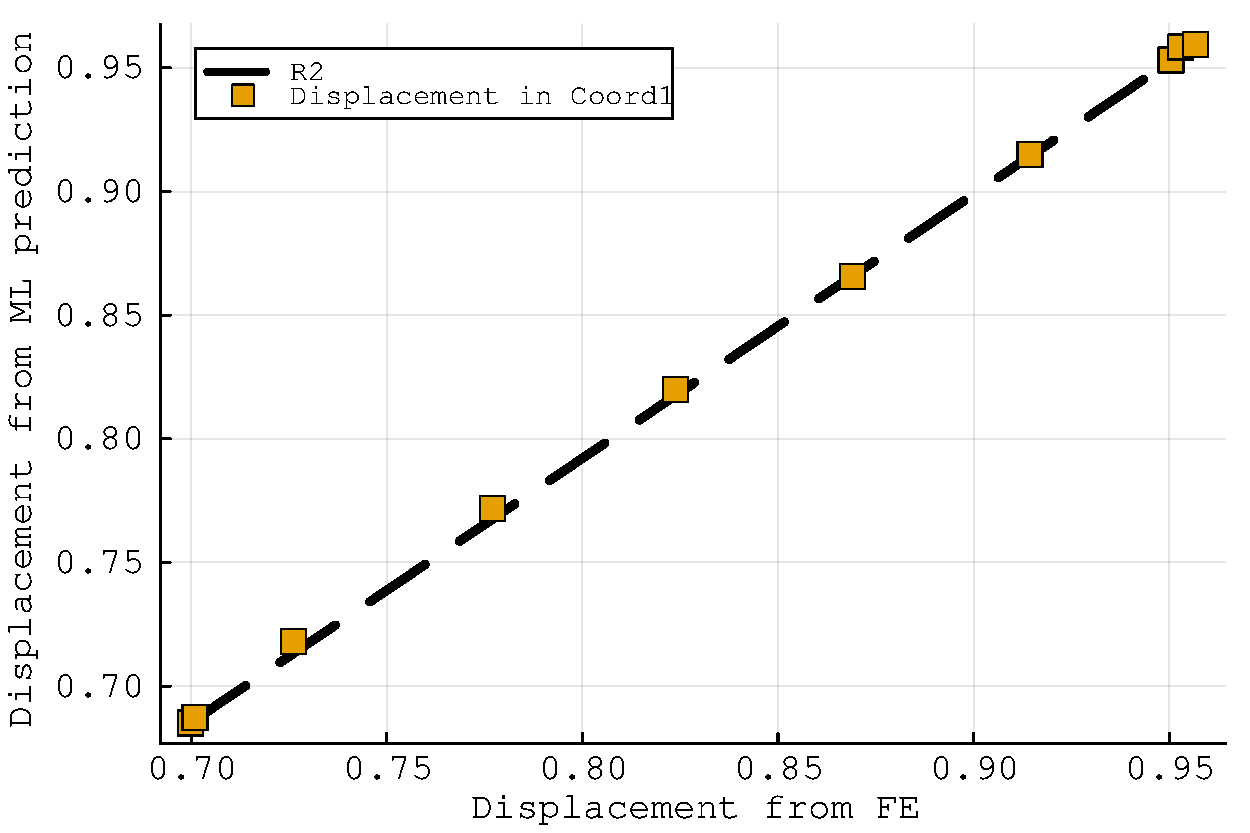
\includegraphics[width=0.45\linewidth]{Figures/NeuralNetworkStudy/R2_Coord1.pdf}}
  \subfloat[Displacement in the third axis of the coordenate system]{\includegraphics[width=0.45\linewidth]{Figures/NeuralNetworkStudy/R2_Coord3.pdf}}
  \caption{R2 evaluation of the displacements. FE data vs ML predicted output}
\end{figure}



Then, we can plot the loss function during the training to visualize the downward tendency.

\begin{figure}
  \begin{center}
    \includegraphics[width=0.6\textwidth]{Figures/NeuralNetworkStudy/Loss_1.pdf}
  \end{center}
  \caption{Loss function during the training for the best performant neural network configuration}\label{fig:}
\end{figure}


